\chapter{架构实现}

\section{架构优势}

\begin{myeasylist}{itemize}
& 独立的元数据服务
& 节点内双控架构
& 全局负载均衡
& 控制路径和数据路径分离
& 全用户态,用了spdk的libnvme和nvmf
& kernel bypass
\end{myeasylist}

\section{Reactive Manifesto}

\mygraphics{../imgs/arch/reactive-traits.png}

作为实现方法,怎么理解message-driven。

如何突破传统架构的束缚,就成为摆在华为存储团队面前最大的挑战。为此,在OceanStor Dorado V6项目开始之际,
华为存储团队就确定了攻克方向:\hl{将Scale-Up和Scale-Out进行融合,设计出一种兼具两者优势的全新架构},
这个目标激发了团队成员巨大动力。

\subsection{Responsive}

\subsection{Resilient}

有无单点故障?

\subsection{Elastic}

scale up, scale out

节点内多控架构,可以扩展到更多core上。

集群扩容,阵列有扩控等操作。

单卷大小和性能

\section{RAID分析}

% RAID分析作为架构驱动力

% 假设和信念
% \begin{enumbox}
% \item 云是新常态
% \item 数据资产是战略资源
% \item 全闪是大势所趋
% \end{enumbox}

\subsection{依赖性}

\mygraphics{../imgs/arch/feature-deps.png}

% \begin{enumbox}
% \item ETCD
% \item SPDK(Driver/Target)
% \item KV
% \end{enumbox}

\section{架构演进}

新设计解决了什么老问题?
\begin{enumbox}
\item 单卷的水平扩展问题
\item IO path上的数据转发问题
\item 单卷大小的限制(支持大卷)
\item chkinfo是动态大小的,副本数、EC配置
\item ***
\item allocate性能低,影响精简配置和COW性能
\item 每个节点导出core、disk等资源,进行全局调度(均衡)
\item 灵活的MM
\item thread local影响CPU利用率
\item ***
\item 重新调整数据布局
\item 底层chunk对象依然不是跨卷的
\item ***
\item COW: volume和snapshot共享对象
\item ***
\item table1/table2实现过于复杂的问题
\item disk md and slots
\item coroutine难于调试
\item ***
\item 多网络
\item MULTIPATH
\item IPv6
\end{enumbox}

\subsection{支持大卷}

\subsection{单卷的水平扩展}

\subsection{IO路径的数据转发}

\subsection{全局负载均衡}

\subsection{更多信息记录在ETCD上}

更灵活,突破结构约束。

\begin{enumbox}
\item 卷的快照树
\item xattr
\end{enumbox}

\subsection{支持EC}

\section{模块}

分布式系统架构通常包括几个部分:client、mds、cds。分别对应什么?
\begin{center}
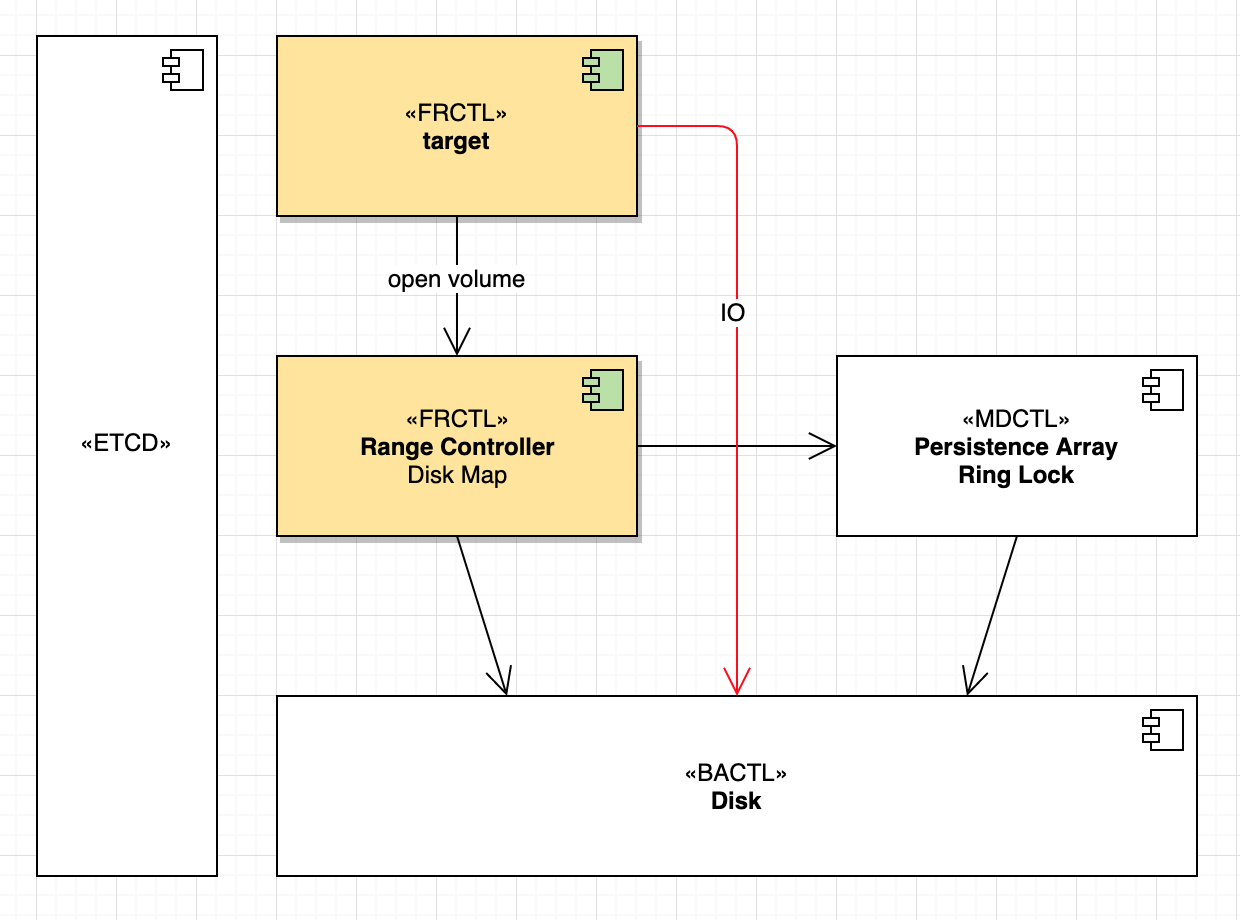
\includegraphics[width=10cm]{../imgs/arch/modules.png}
\end{center}

target到bactl,有两条路径,视是否通过range ctl而定。如果不通过range ctl(rangectl bypass),数据流可直达后端存储,
实现控制流和数据流分流的目的。同时降低了转发成本。

\begin{center}
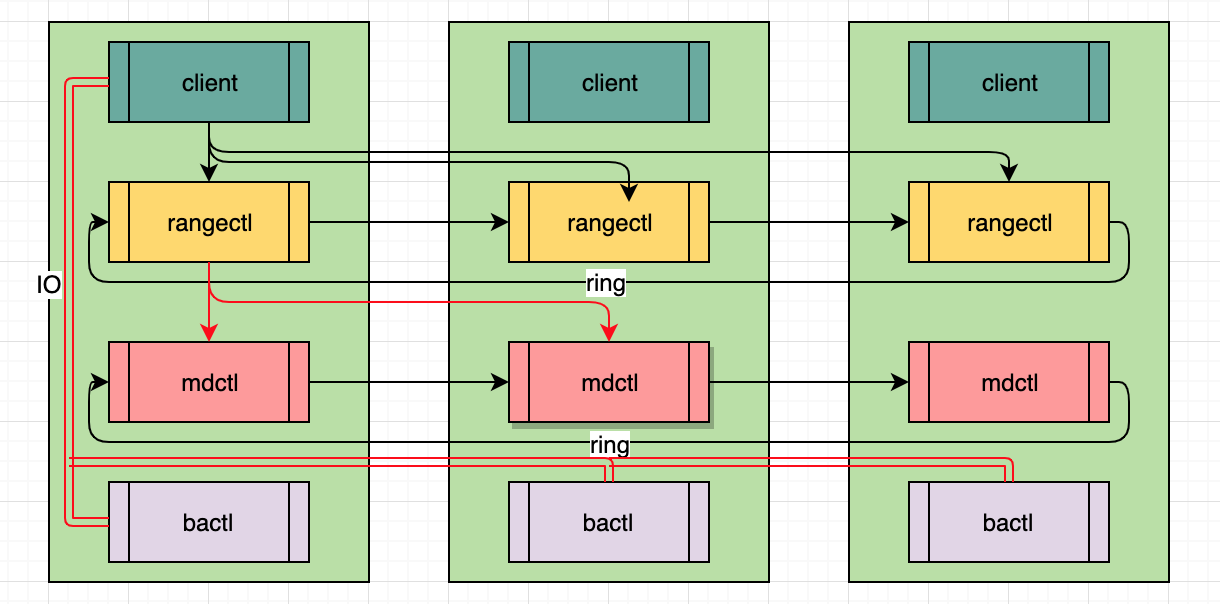
\includegraphics[width=10cm]{../imgs/message-flow.png}
\end{center}

问题集:
\begin{enumbox}
\item 为什么range ctl和mds是分离的进程?
\item vss是否必要?
\item ***
\item io路径是什么?
\item 副本一致性是如何实现的?
\item IO和Recovery之间如何同步?
\end{enumbox}

\subsection{TgtCtl}

\subsection{FRCTL}

target如何与分布式卷相连?

\subsection{RangeCtl}

token是向range ctl获取的,粒度为chunk。range ctl上每个chunk维护有token计数器。

token里包含了每个副本的位置信息,这是向mds请求得到的。

client并不与mds直接通信。分离fr和mds为两个进程,一是可以指定不同的core;二,便于debug。

\begin{center}
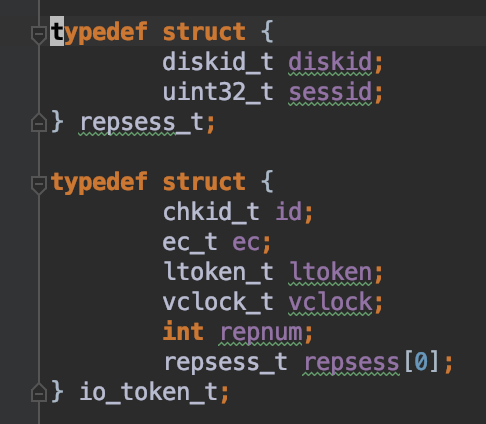
\includegraphics{../imgs/token.png}
\end{center}

range ctl和mds都在hash ring上。都采用了hash机制来定位目标节点。
所以\hl{有两个hash ring:range ctl和mds}。两个ring都通过mds master来维护。
ring的节点结构是什么?node and core?
\begin{center}
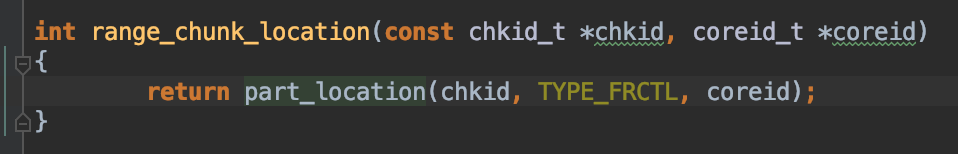
\includegraphics[width=10cm]{../imgs/chunk-location.png}
\end{center}

partition是range ctl和mdctl共用模块。range ctl目前归属frctl。

lease机制目前没用,如果需要把range ctl放置到session所在的位置(一个volume的所有range都在一个节点上?),
可以选用lease机制,而不用dht机制。怎么理解session?

一旦ring结构发生变化,会有什么影响?SSAN通过epoch来管理ring结构的变化。

ring上节点负载均匀性如何?

ring lock有什么用?在mds master上维护状态,处理ring发生变更的情况。
是否可通过引入epoch实现同样的功能?

GFM?解决全局同一视图的问题。

如何识别和处理stale消息?

\subsection{MDCTL}

hash ring上有一个节点充当master角色。如何选主,如何保持其唯一性?
通过etcd lock实现。

\subsection{BACTL}

\mygraphics{../imgs/suzaku/disk-connect.png}

redis的数据模型?

diskid是全局的,在etcd上有目录。

diskmd磁盘访问接口,支持libnvme驱动。

需要管理物理内存,如hugepage和memory pool。

NVMe/RDMA需要访问物理内存地址(v2p)。

\section{数据模型}

\mygraphics{../imgs/cluster-virt.png}

从\hl{资源的生命周期模型}开始思考。资源包括:\hl{集群、节点、core、磁盘、pool、volume、snapshot}等,以及内部资源。

\subsection{Cluster}

\subsection{Pool}

Pool是对磁盘的横向物理划分。

\subsection{Node}

Node是Process、Core、Disk等资源的合集。利用Core的方式是个亮点。

增删节点是重大事件

\subsection{Disk}

Disk导出,分配过程可以进行全局调度。

调度器位于md ctl。md ctl负责管理chkid到disk id的映射关系。
\todo{diskid类型}diskid采用16bit整数是否太小?

diskmap.c,不宜放入bactl。bactl所有API都带diskid,针对单盘进行。

怎么做到每个副本属于不同的节点的呢?

如何管理diskmap的版本呢?

\hl{数据分布的均匀性}: 节点和磁盘两种粒度

tier and cache?

负载均衡

\subsection{Volume}

\begin{center}
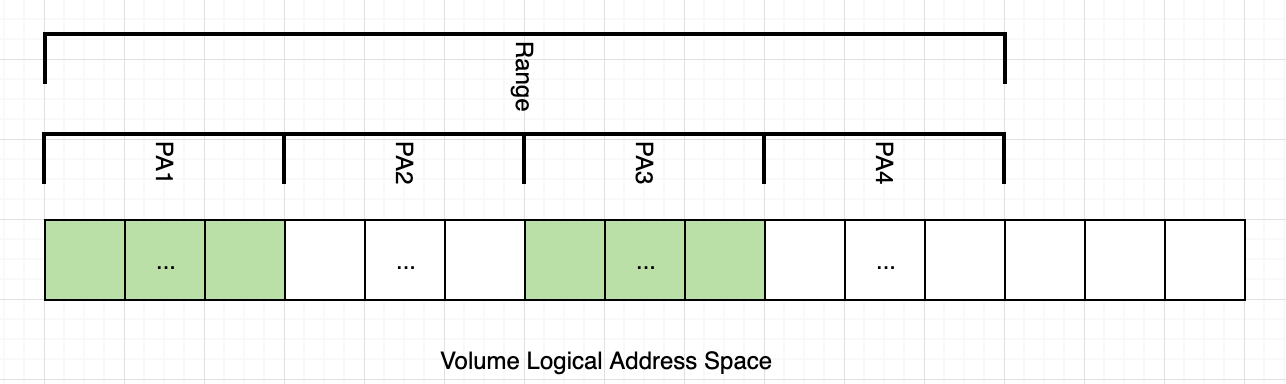
\includegraphics[width=10cm]{../imgs/volume-addressspace.png}
\end{center}

vss包括4个range,range包括4个pa,pa包括固定数目的chunk。pa和chunk都是4M大小。
\todo{vss是否必要}vss是否必要,还是增加了设计复杂度?

\begin{center}
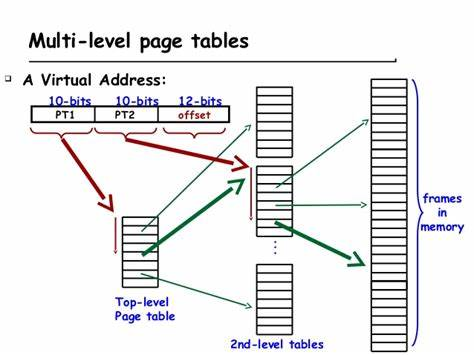
\includegraphics[width=10cm]{../imgs/oos/pagetable.jpeg}
\end{center}

采用两层元数据,第一层有一个PA对象,记录指向第二层PA对象;
第二层的PA对象按需分配,记录指向卷地址空间chunk对象。由此可推算最大卷的大小。

两层元数据,etcd指向顶层对象。每个对象属于一个卷,
因为不是一般的对象系统,\hl{在快照的情况下,无法直接共享}。

\hrulefill

功能
\begin{enumbox}
\item TP
\item Recovery
\item Balance
\item QoS
\item ***
\item EC
\item Dedup
\item Compress
\item ***
\item RC
\end{enumbox}

\subsection{Snapshot}

分析各种操作的复杂度,包括空间和时间。

\hrulefill

COW的问题
\begin{enumbox}
\item 影响写性能
\item Rollback慢
\item clone卷慢,scan snap tree。snapshot也可执行flatten
\end{enumbox}

snap头包含什么指针?

映射表的管理粒度,是chunk还是page?范围,是全局还是私有?

如何共享底层对象?

COW一次读,两次写

ROW一次读,一次写

ROW,两层元数据?

\hrulefill

SSAN的snapshot实现。

consistency group

\section{ID}

\subsection{Pool ID}

\subsection{NID}

参考nodeid.c。

\subsection{CoreID and DiskID}

coreid内置nid,diskid通过d2n\_nid函数映射到nid。都需要两次映射进行定位。

\hl{core和disk都是归属于node的资源},导出进行全局调度,why不用同一种形式?

考虑支持\hl{服务器之间的disk漂移特性}。

\subsection{Volume ID}

\mygraphics{../imgs/arch/volume-meta.png}

卷有两层元数据,由此可以算出卷的最大大小。支持精简配置。

\subsection{Chunk ID}

\section{ETCD}

\subsection{etcd idx}

更新etcd的KV是个cas过程,避免并发冲突。

\subsection{Pool}

\mygraphics{../imgs/etcd/etcd-pool.png}

\subsection{Metadata}

\mygraphics{../imgs/etcd/etcd-metadata.png}

\subsection{Coreid and Diskid}

\mygraphics{../imgs/etcd/etcd-instance.png}

两个hash ring:rangectl and mdctl。

\subsection{Network}

\mygraphics{../imgs/etcd/etcd-network.png}

\section{MDS}

\subsection{Leader Election}

\subsection{Cluster Map}

\mygraphics{../imgs/partition/mds-master.png}

\mygraphics{../imgs/partition/partition-update.png}

mds master维护两个hash ring信息,如有变化更新到etcd上,slave定期poll该信息。

\subsection{Disk Map}

disk scanner

\section{Range Ctl}

\subsection{如何定位RangeCtl的位置?}

lich里用到了广播机制和第一副本作为卷控的约定。

\subsection{md-chunk-load}

如何定位一个chunk的chkinfo信息?

\mygraphics{../imgs/partition/md-chunk-load.png}

\section{IO}

\subsection{Allocate}

diskmap

\subsection{Write}

\subsection{Read}

\section{Recover}

\mygraphics{../imgs/rangectl/chunk-get-token.png}

io内恢复

\mygraphics{../imgs/rangectl/recovery-file.png}

外部线程触发恢复,\hl{io、恢复、平衡都是rangectl协作}进行。

需求
\begin{myeasylist}{itemize}
& 每个pool扫描属于本pool的卷,一个卷由一个节点负责
& 节点故障和磁盘故障的scan阶段不同,恢复阶段相同
& 可以start/stop/restart pool的恢复任务
& 可以实时获取恢复进度
& 可以设定卷的恢复优先级
& 可以设定恢复QoS
& 按rangectl分组
& 批量发送
& 修复失败加入fail list,后头再处理
\end{myeasylist}

\hrulefill

HOWTO

\mygraphics{../imgs/task/recovery-thread-structure.png}

启动恢复的主线程

有故障时,唤醒影响所及的pool恢复线程。disk故障可以定向修复,也可以先同节点故障。

每个存储池有存储池的主线程,负责pool内所有卷的修复。
分为scan和recover多阶段,可以组织成pipeline的结构。

scan出所有的chkid,给对应的rangectl发送请求,可以在一次请求中发送多个chkid。

每个rangectl维护一个队列。

\section{Balance}
